\chapter{Grobe Zeit- und Ressourcenplanung}
% \label{Kap3}

\begin{itemize}
    \item \textbf{November 2020 bis Dezember 2020:} Kapitel 2, 3 (ca. 40\% der Arbeit)
    \item \textbf{Januar 2021:} Kapitel 4 (ca. 35\% der Arbeit)
    \item \textbf{Februar 2021:} Kapitel 5 (ca. 10\% der Arbeit)
    \item \textbf{März 2021:} Kapitel 1, 6, 7 (ca. 15\% der Arbeit)
\end{itemize}
% \section{Bilder}

% Natürlich können auch Grafiken und Bilder eingebunden werden, siehe z.\,B. Abbildung~\ref{Kap2:NasaRover}.

% \begin{figure}[ht]
%   \centering
%   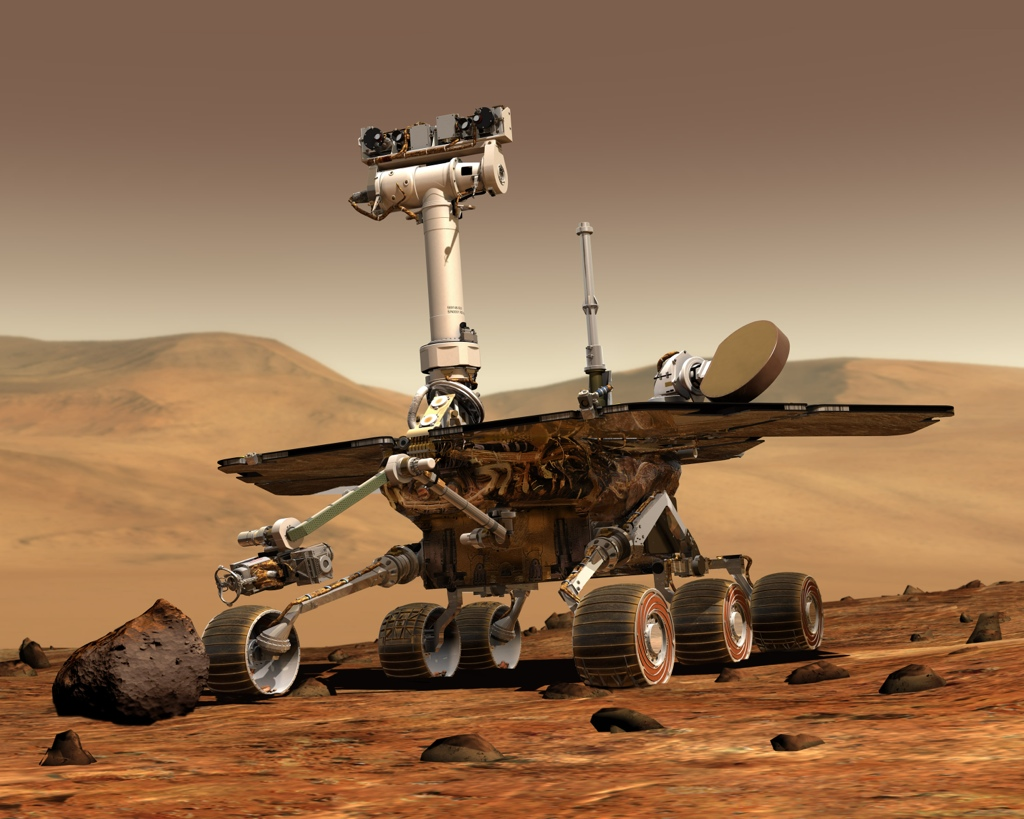
\includegraphics[width=6cm]{kapitel3/nasa_rover}
%   \caption{Ein Nasa Rover}
%   \label{Kap2:NasaRover}
% \end{figure}

% Man kann sich auch selbst ein Makro für das Einfügen von Bildern schreiben:

% \bild{kapitel3/modell_point_to_point}{6cm}{Point to Point}

% \begin{sidewaysfigure}
%  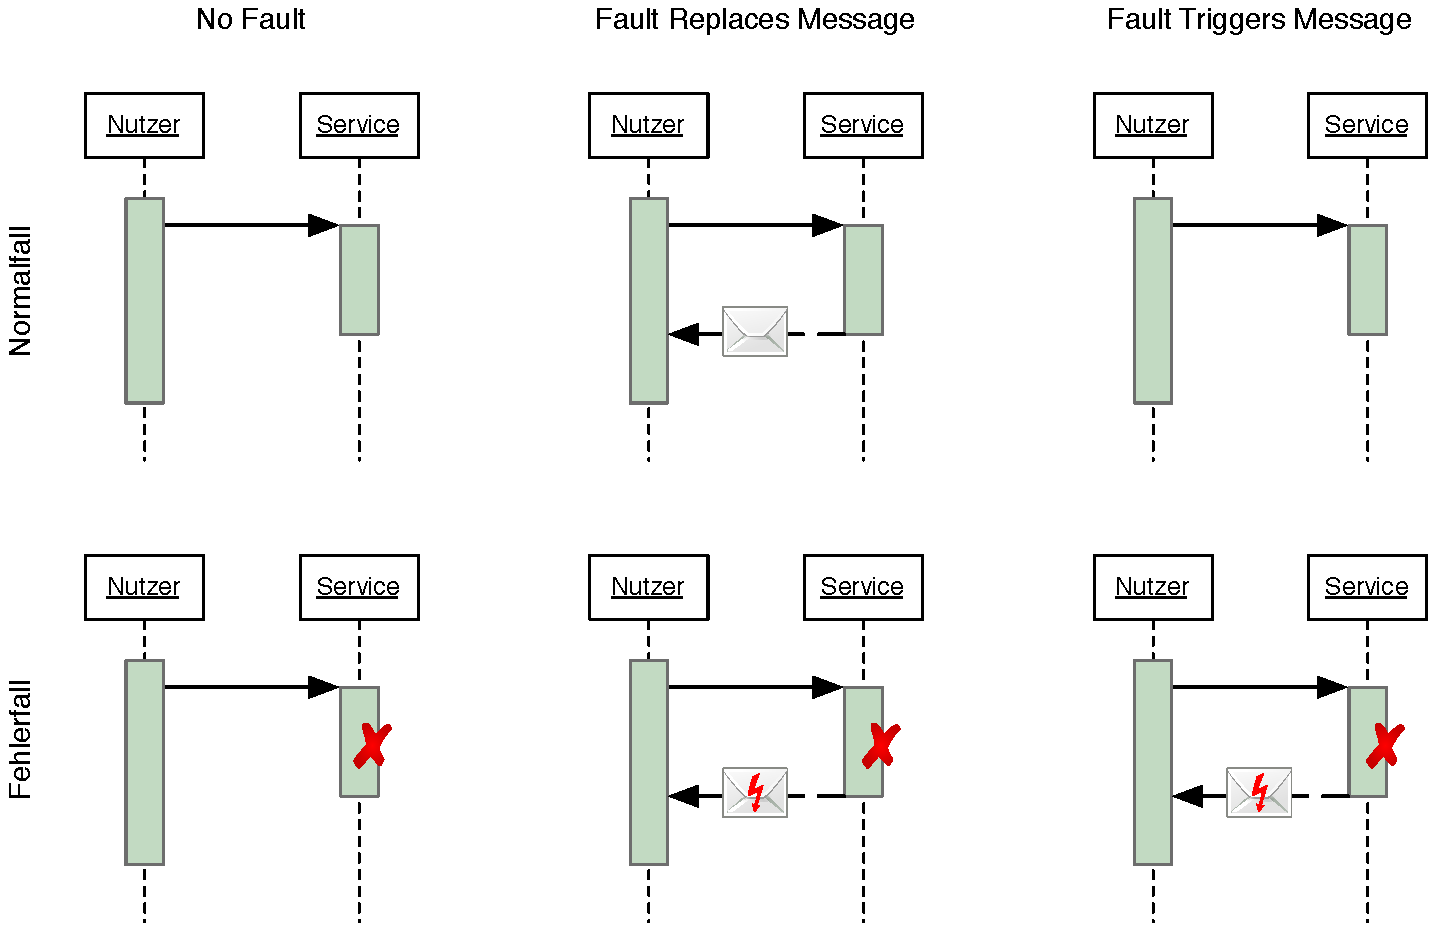
\includegraphics[width=22cm]{kapitel3/ws-wsdl20-fehler}
%   \caption{Sehr große Grafiken kann man drehen, damit sie auf die Seite passen}
%   \label{Kap2:wsdl-fehler}
% \end{sidewaysfigure}

% \clearpage % Alle Bilder, die bisher kamen ausgeben


% \section{Formelsatz}

% Eine Formel gefällig? Mitten im Text $a_2 = \sqrt{x^3}$ oder als eigener Absatz (siehe Formel~\ref{Formel}):

% \begin{equation}
% \begin{bmatrix}
%    1 &  4 &  2 \\
%    4 &  0 & -3
% \end{bmatrix}
%         \cdot
% \begin{bmatrix}
%    1 &  1 &  0 \\
%   -2 &  3 &  5 \\
%    0 &  1 &  4
% \end{bmatrix}
%        {=}
% \begin{bmatrix}
%   -7 &  15 &  28 \\
%    4 &   1 & -12
% \end{bmatrix}
% \label{Formel}
% \end{equation}


% \section{Sourcecode}

% Man kann mit Latex auch ganz toll Sourcecode in den Text aufnehmen.

% \subsection{Aus einer Datei}

% \lstinputlisting[firstline=2,language=Java,caption={Crypter-Interface},label=lst:CrypterInterface]{\srcloc/Crypter.java}


% \subsection{Inline}

% \begin{lstlisting}[language=Java,caption=Methode checkKey()]
%     /**
%      * Testet den Schlüssel auf Korrektheit: Er muss mindestens die Länge 1
%      * haben und darf nur Zeichen von A-Z enthalten.
%      *
%      * @param key zu testender Schlüssel
%      * @throws CrypterException wenn der Schlüssel nicht OK ist.
%      */
%     protected void checkKey(Key key) throws CrypterException {

%         // Passt die Länge?
%         if (key.getKey().length == 0) {
%             throw new CrypterException("Der Schlüssel muss mindestens " +
%                     "ein Zeichen lang sein");
%         }

%         checkCharacters(key.getKey(), ALPHABET);
%     }
% \end{lstlisting}


% \section{Anforderungen}

% Anforderungen im Format des Volere"=Templates (Snowcards) \autocite{Volere} können per Makro eingefügt werden. Das Label wird automatisch mit der Nummer erstellt, d.\,h. Sie können auf die Tabelle mit dieser referenzieren (siehe \autoref{F52}).

% \snowcard % Snowcard einbinden (Anpassungen in titelblatt.tex)
%    {F52} % Nummer des Requirements
%    {F} % Art
%    {Hoch} % Priorität
%    {User Authentifizierung} % Titel
%    {Interview mit Abteilungsleiter} % Herkunft (Optional)
%    {F12} % Konflikte (Optional)
%    {Der Benutzer ist in der Lage sich über seinen
%     Benutzernamen und sein Passwort am System anzumelden} % Beschreibung
%    {Ein Benutzer kann sich mit seinem firmenweiten Benutzernamen und
%    Passwort über die Anmeldemaske anmelden und hat Zugriff auf die
%    Funktionen des Systems} % Fit-Kriterium (Optional)
%    {Benutzerhandbuch des Altsystems} % Material (Optional)

% Ebenso können Sie nicht"=funktionale Anforderungen mit Hilfe von Quality Attribute Scenarios (vgl. \autoref{NF11}) darstellen. Zu Details siehe \autocite{Barbacci2003}.

% \qas % Quality-Attribute Scenario einbinden (Anpassungen in titelblatt.tex)
%    {NF11} % Nummer des Requirements
%    {Hoch} % Priotität
%    {Performance des Jahresabschlusses} % Titel
%    {Endbenutzer} % Quelle
%    {Startet einen Jahresabschluss} % Stimulus
%    {Buchhaltungssystem} % Artefakt
%    {Das System befindet sich im normalen Betriebszustand} % Umgebung
%    {Jahresabschluss ist durchgeführt und kann als PDF abgerufen werden} % Antwort
%    {10 Minuten} % Antwort-Maß

% Die Abgrenzung von funktionalen und nicht-funktionalen Anforderungen ist nicht immer einfach und bereitet manchen Studierenden Probleme. Als Hilfestellung kann die von der ISO25010 \autocite{ISO25010} zur Verfügung gestellte Liste dienen, siehe \autoref{kapitel3/iso25010}.

% \bild{kapitel3/iso25010}{14cm}{Qualitätsmodell für Software-Produkte nach ISO25010}

% \citeauthor{Bass2003} listen in \autocite{Bass2003} eine ähnliche Liste von Kategorien für nicht-funktionalen Anforderungen auf, die ebenfalls als Richtschnur dienen kann. Diese sind:

% \begin{itemize}
%   \item \textit{Verfügbarkeit} \textit{(availability)} -- umfasst Zuverlässigkeit (reliability), Robustheit (robustness), Fehlertoleranz (fault tolerance) und Skalierbarkeit (scalability)
%   \item \textit{Anpassbarkeit} \textit{(modifiability)}, umfasst Wartbarkeit (maintainability), Verständlichkeit (understandability) und Portabilität (portability).
%   \item \textit{Performanz} \textit{(performance)}
%   \item \textit{Sicherheit} \textit{(security)}
%   \item \textit{Testbarkeit} \textit{(testability)}
%   \item \textit{Bedienbarkeit} \textit{(usability)}
% \end{itemize}
